We have implemented our approach in a prototype and compared it with the related 
approaches \texttt{refinepoly}~\cite{singh2019beyond}, \texttt{deepSRGR}~\cite{yang2021improving}, and \deeppoly{}~\cite{singh2019abstract}. 
The approaches  \texttt{refinepoly} and \texttt{deepSRGR} do the refinement on \deeppoly{}. We also compare 
our tool with state-of-the-art tools $\alpha - \beta$-Crown~\cite{alphabetacrown} and oval~\cite{ovaltool}. 
The $\alpha - \beta$-Crown tool has achieved the 1st and oval 3rd rank in
2nd International Verification of Neural Networks Competition (VNN-COMP'21). 
We use the MNIST \cite{deng2012mnist} for our evaluation.    
\subsection{Implementation}
We have implemented our tool in \texttt{C++} programming language. Our approach relies on \deeppoly{}, so, 
we also have implemented \deeppoly{} in \texttt{C++}. We are using a \texttt{C++} interface of gurobi solver 
to check the satisfiability or to solve an optimization query. 

\subsection{Benchmarks}
We are using the MNIST~\cite{deng2012mnist} dataset to check the effectiveness of our tool. 
We are using 11 different fully connected feedforward neural networks with \relu{} activation as shown in table~\ref{tb:nndetail}.
These benchmarks are taken from the \deeppoly{}'s paper~\cite{singh2019abstract}. 
The input and output dimensions of each network are $784$ and $10$ respectively. 
The authors of \deeppoly{} used projected gradient descent (PGD)~\cite{dong2018boosting}
and DiffAI~\cite{mirman2018differentiable} for adversarial training. Table \ref{tb:nndetail} contains the defended network i.e.
trained with adversarial training as well as the undefended network. The last column of the table \ref{tb:nndetail}
shows tool's name by which the defended networks are trained.  

The predicate $P$ on the input layer is created using the input image $\boldsymbol{im}$ and user-defined parameter $\epsilon$. 
We first normalize each pixel of $\boldsymbol{im}$ between $0$ and $1$, then create 
$P = \Land_{i=1}^{|l_0|} im(i)-\epsilon \leq x_{0i}\leq im(i)+\epsilon$, such that the lower and upper bound of each pixel
should not exceed $0$ and $1$ respectively. The predicate $Q$ on the output layer is created using the network's output.    
Suppose the predicted label of $\boldsymbol{im}$ on network $N$ is $y$, then $Q = \Land_{i=1}^{|l_k|} x_{ki} < y$, where $i \neq y$. 
One query instance $\langle N,P,Q \rangle$ is created for one network, one image and one epsilon value. 
In our evaluation, we took $11$ different networks, 8 different epsilons, and 100 different images. The 
total number of instances is computed to $8800$. However, there are 128 instances for which the network's predicted
label differs from the image's actual label. we avoided such instances, so, there is a total of $8672$ benchmark instances
under consideration.   
Whenever our tool found a counter-example on $\langle N,P,Q \rangle$,
it denormalizes it into an image by rounding the float values 
and checks for counter-example by executing $N$ on the denormalized image.
If found counter-example then the tool reports it, otherwise, the tool reports unknown.



\begin{table}
    \centering
    \begin{tabular}{c|c|c|c}
        \hline
        \textbf{Neural Network} & \textbf{\#hidden layers} & \textbf{\#activation units} & \textbf{Defensive training} \\
        \hline
        $3\times 50$ & 2 & 110 & None \\
        $3\times 100$ & 2 & 210 & None  \\
        $5\times 100$ & 4 & 410 & None  \\
        $6\times 100$ & 5 & 510 & DiffAI \\
        $9\times 100$ & 8 & 810 & None  \\
        $6\times 200$ & 5 & 1010 & None  \\
        $9\times 200$ & 8 & 1610 & None  \\
        $6\times 500$ & 6 & 3000 & None  \\
        $6\times 500$ & 6 & 3000 & PGD, $\epsilon = 0.1$ \\
        $6\times 500$ & 6 & 3000 & PGD, $\epsilon = 0.3$ \\
        $4\times 1024$ & 3 & 3072 & None  \\
        \hline
    \end{tabular}
    \caption{Neural networks details}
    \label{tb:nndetail}
\end{table}

\subsection{Results}
We conducted the experiments on a machine with \texttt{64GB RAM, 2.20 GHz Intel(R) Xeon(R) CPU E5-2660 v2}
processor with CentOS Linux 7 operating system. 
To make a fair comparison between the tools, we provide only a single \texttt{CPU} for each benchmarks instances for each tool. 
The approaches \deeppoly{}, \texttt{refinepoly}, and \texttt{deepSRGR} are incomplete and do not report the counter-example. 
Our approach is a complete approach. We compare our approach's \texttt{verified} only instances with incomplete approaches. 
Figure~\ref{res:milp_with_milp} shows the comparison with the help of the cactus plot. Our approach performs well 
in terms of the verified number of instances as well as in terms of time in comparison to the above incomplete approaches. 
We are also comparing with state of the arts to check the effectiveness of our approach globally.
Table~\ref{tb:soacomparison} shows that our tool is verifying $180$ and $190$ benchmarks which $\alpha -\beta$-CROWN and 
\texttt{oval} respectively are not able to verify. In addition to this, our tool verifies $172$ unique instances 
that neither $\alpha -\beta$-CROWN nor \texttt{oval} is able to verify.  
Despite it, $\alpha - \beta-$Crown and \texttt{oval} are verifying more benchmarks in comparison to our tool. 
Although the total time taken by both state of the arts is higher than our tool as shown in figure~\ref{res:milp_with_milp}. 


\begin{table}
    \centering
    \begin{tabular}{|c|c|c|c|}
        \hline
        -  & Not verified by oval & Not verified by $\alpha - \beta$-CROWN & Not verified by both \\
        \hline
        Verified by our tool & 190 & 180 & 172 \\
        \hline
    \end{tabular}
    \caption{Comparison with $\alpha - \beta$-CROWN and Oval}
    \label{tb:soacomparison}
\end{table}



\begin{figure}
    \centering
    
\begin{tikzpicture}
    \begin{axis}[
        xlabel={Number of benchmarks},
        ylabel={log(time)},
        width=13cm,
        height=9cm,
        xmin=0, xmax=7000,
        ymin=0, ymax=25,
        xtick={0,1000,2000,3000,4000,5000,6000,7000},
        ytick={0,5,10,15,20,25},
        legend pos=south east,
        legend entries={drefine, deeppoly, deep\_SRGR, refinepoly, drefine\_verified, alpha\_beta, oval, cegar\_nn},
        ymajorgrids=true,
        xmajorgrids=true,
        grid style=dashed,
    ]
    \addplot[
        color=blue
    ] 
    table {fig/drefine_data.txt};
    
    \addplot[
        color=red
    ] 
    table {fig/deeppoly_data.txt};

    \addplot[
        color=orange
    ] 
    table {fig/deepsrgr_data.txt};

    \addplot[
        color=green
    ] 
    table {fig/refinepoly_data.txt};

    \addplot[
        color=violet
    ]
    table {fig/drefine_verified_data.txt};
    
    \addplot[
        color=purple
    ]
    table {fig/alpha_beta_data.txt};

    \addplot[
        color=brown
    ]
    table {fig/oval_data.txt};

    \addplot[
        color=gray
    ]
    table {fig/four_class_data.txt};

    \end{axis}

\end{tikzpicture}
    \caption{Cactus plot with related techniques}
    \label{res:milp_with_milp}
\end{figure}


Figure~\ref{res:ep:milp_with_milp} shows the comparison with respect to different epsilon values. 
At $\epsilon=0.005$, the performance of all the tools is almost the same. As the value of epsilon increases, the 
performance of tools can be seen clearly. Here also we are performing better than the approaches \deeppoly{}, 
\texttt{refinepoly}, and \texttt{deepSRGR},
while $\alpha - \beta -$Crown and \texttt{oval} are performing better than our tool. 
The average number of marked neurons on the finished benchmarks instances is $31$. 

% Figures \ref{res:milp_with_milp} and \ref{res:ep:milp_with_milp} shows that we are performing better in compare to
% the most related techniques \deeppoly{}, \texttt{refinepoly} and \texttt{deepSRGR}. 

\begin{figure}
    \centering
    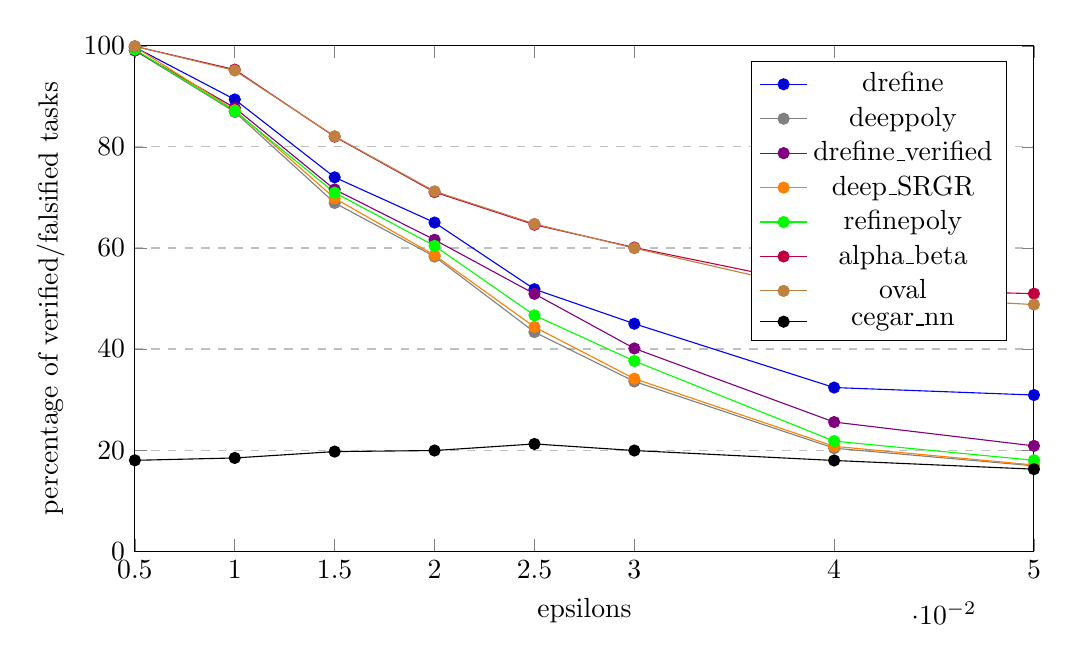
\begin{tikzpicture}
    \begin{axis}[
        xlabel={epsilons},
        ylabel={percentage of verified/falsified tasks},
        width=13cm,
        height=8cm,
        xmin=0.005, xmax=0.05,
        ymin=0, ymax=100,
        xtick={0.005,0.01,0.015,0.02,0.025,0.03,0.04,0.05},
        ytick={0,20,40,60,80,100},
        legend pos=north east,
        legend entries={drefine,deeppoly, drefine\_verified, deep\_SRGR, refinepoly, alpha\_beta, oval, cegar\_nn},
        ymajorgrids=true,
        grid style=dashed,
    ]
    \addplot+[
        color=blue,
        mark=*,
    ]
    coordinates {
        (0.005,99.72)(0.01,89.39)(0.015,73.98)(0.02,65.03)(0.025,51.84)(0.03,45.01)(0.04,32.38)(0.05,30.9)
    };

    \addplot[
        color=gray,
        mark=*,
    ]
    coordinates {
        (0.005,99.07)(0.01,86.9)(0.015,68.91)(0.02,58.3)(0.025,43.35)(0.03,33.58)(0.04,20.38)(0.05,16.89)
    };

    \addplot[
        color=violet,
        mark=*,
    ]
    coordinates {
        (0.005,99.07)(0.01,87.73)(0.015,71.58)(0.02,61.62)(0.025,50.92)(0.03,40.12)(0.04,25.55)(0.05,20.84)
    };

    \addplot[
        color=orange,
        mark=*,
    ]
    coordinates {
        (0.005,99.8)(0.01,87.26)(0.015,69.83)(0.02,58.57)(0.025,44.37)(0.03,34.13)(0.04,20.75)(0.05,17.06)
    };

    \addplot[
        color=green,
        mark=*,
    ]
    coordinates {
        (0.005,99.26)(0.01,87.08)(0.015,70.94)(0.02,60.42)(0.025,46.67)(0.03,37.63)(0.04,21.78)(0.05,17.99)
    };

    \addplot[
        color=purple,
        mark=*,
    ]
    coordinates {
        (0.005,99.9)(0.01,95.29)(0.015,82.02)(0.02,71.05)(0.025,64.60)(0.03,60.09)(0.04,51.98)(0.05,50.96)
    };

    \addplot[
        color=brown,
        mark=*,
    ]
    coordinates {
        (0.005,99.9)(0.01,95.11)(0.015,82.1)(0.02,71.21)(0.025,64.76)(0.03,59.96)(0.04,50.92)(0.05,48.8)
    };

    \addplot[
        color=black,
        mark=*,
    ]
    coordinates {
        (0.005,17.98)(0.01,18.45)(0.015,19.71)(0.02,19.92)(0.025,21.22)(0.03,19.92)(0.04,17.95)(0.05,16.23)
    };


    \end{axis}

\end{tikzpicture}
    \caption{Epsilon wise comparison with related techniques}
    \label{res:ep:milp_with_milp}
\end{figure}
